\documentclass[12pt, twoside, a4paper]{report}

\author{Mayank Jatav}
\usepackage{mathptmx, lettrine}
\usepackage{mathtools,amsmath}
\usepackage{gensymb}
% Beautiful Math Font
\usepackage{eulervm}
\usepackage{mathptmx, lettrine}
\usepackage{mathtools,amsmath}
\usepackage{tabularray}
\usepackage{gensymb}
\usepackage{booktabs}
\usepackage{multirow}
\usepackage{amsfonts}

% Table Options
\usepackage{array, longtable, subcaption, multirow, tabularx, booktabs}
\captionsetup{%
	figurename=Figure
	tablename=Table
}
% Graphics and Figure Options
\usepackage{graphics, float, xcolor}

% Aligning/Formatting Equations
\usepackage{amsmath}

% Typeset Text
\usepackage{microtype}

% Customize Lists
\usepackage{enumitem}%\setlist[itemize]{noitemsep, topsep=0pt}
\setlist[itemize]{topsep=2pt}
\setlist[enumerate]{topsep=2pt}

\usepackage{lscape, rotating, layout}
\usepackage[a4paper, left=20mm, right=20mm, top=30mm, bottom=30mm]{geometry}	% Online
%\usepackage[a4paper, left=35mm, right=20mm, top=30mm, bottom=30mm]{geometry} 	% Print

% Fancy Header
\usepackage{fancyhdr}
\fancyhf{}
\pagestyle{fancy}
\renewcommand{\headrulewidth}{0.4pt}
\renewcommand{\footrulewidth}{0.4pt}
\setlength{\headheight}{3mm}
\setlength{\footskip}{10mm}

% Referencing Options
\usepackage{cite}
\usepackage{lscape}
% Blank Pages - Empty Header
\usepackage{emptypage}
% Chapter Title Design
\usepackage[T1]{fontenc}
\usepackage[charter]{quotchap}

% Hyphenation
\usepackage{hyphenat}
\usepackage[english]{babel}

% Color HyperLinks
\definecolor{darkpastelgreen}{rgb}{0.01, 0.75, 0.24}
\usepackage{hyperref, url}

% ...existing code...
\usepackage{titlesec}
\titlespacing*{\section}{0pt}{0.5em}{0.5em}
\titlespacing*{\subsection}{0pt}{0.5em}{0.5em}
\titlespacing*{\subsubsection}{0pt}{0.5em}{0.5em}
% ...existing code...

% Online
\hypersetup{colorlinks=true, linkcolor=blue, citecolor=darkpastelgreen, filecolor=magenta, urlcolor=blue}
% Print
% \hypersetup{colorlinks=false, linkcolor=black, filecolor=black, urlcolor=black}
% Acronyms/Glossary
\usepackage[nopostdot, style=super, nonumberlist, toc, automake, acronym]{glossaries}
\makeglossaries

\renewcommand{\glsnamefont}[1]{\textbf{#1}}
\newacronym{ref}{ref}{Reference}
\newacronym{CNN}{CNN}{Convolutional Neural Network}
\newacronym{ViT}{ViT}{Vision Transformer}

% Macro
\providecommand{\keywords}[1]{\textbf{\textit{Keywords---}} #1}

% Big O Notation
\newcommand{\bigO}[1]{\ensuremath{\mathop{}\mathopen{}\mathcal{O}\mathopen{}\left(#1\right)}}

%%%%%%%%%%%%%%%%%%%%%%%%%%%%%%%%%%%%%%%%%%%%%%%%%%%%%%%%%%%%%%%%%%%%%%%%%%%%%%%%%%%%%%%%%%%%%%%%%%%%%%

\parskip 2.5mm		% Space before a new Paragraph
\parindent 0pt		% Indent Paragraphs
\linespread{1.3}	% Space between Lines of the paragraph

\setlength{\headheight}{15pt}

% Initialize Table of Contents, List of Figures and List of Tables
\AtBeginDocument{\addtocontents{toc}{\protect\thispagestyle{empty}}}
\AtBeginDocument{\addtocontents{lof}{\protect\thispagestyle{empty}}}
\AtBeginDocument{\addtocontents{lot}{\protect\thispagestyle{empty}}}

%%%%%%%%%%%%%%%%%%%%%%%%%%%%%%%%%%%%%%%%%%%%%%%%%%%%%%%%%%%%%%%%%%%%%%%%%%%%%%%%%%%%%%%%%%%%%%%%%%%%%%
%%%%%%%%%%%%%%%%%%%%%%%%%%%%%%%%%%%%%%%%%%%%%%%%%%%%%%%%%%%%%%%%%%%%%%%%%%%%%%%%%%%%%%%%%%%%%%%%%%%%%%


\begin{document}

%%%%%%%%%%%%%%%%%%%%%%%%%%%%%%%%%%%%%%%%%%%%%%%%%%%%%%%%%%%%%%%%%%%%%%%%%%%%%%%%%%%%%%%%%%%%%%%%%%%%%%

% Change Page Numbering Format
\pagenumbering{arabic}
\pagestyle{fancy}

% Page Headings and Subheadings with Page Number
% TwoPage
\fancyhead[EL, OR]{\thepage}
\fancyhead[ER]{\nouppercase{\leftmark}}
\fancyhead[OL]{\nouppercase{\rightmark}}
% One Page
%\fancyhead[L, R]{\thepage}

\renewcommand{\sectionmark}[1]{\markright{\thesection\ #1}}
%\lhead{\fancyplain{}{\nouppercase{\rightmark}}}

%%%%%%%%%%%%%%%%%%%%%%%%%%%%%%%%%%%%%%%%%%%%%%%%%%%%%%%%%%%%%%%%%%%%%%%%%%%%%%%%%%%%%%%%%%%%%%%%%%%%%%

% Title Page

\begin{titlepage}
\thispagestyle{empty}

%%%%%%%%%%%%%%%%%%%%%%%%%%%%%%%%%%%%%%%%%%%%%%%%%%%%%%%%%%%%%%%%%%%%%%%%%%%%%%%%%%%%%%%%%%%%%%%%%%%%%%

\begin{table}
	\centering
	\begin{tabular}{c}
		\Large \textbf{Fabrics Classification using Deep Learning} \\
		\& \\
		\Large \textbf{Security Orchestration Automation and Response} \\
		\\
		\\
            \\
		\it Synopsis of the thesis submitted in partial fulfilment \\of the requirements for the degree of	\\
            \\
            \\
           
		\bf Master of Technology	\\
		\\
		\\
		
		\it by	\\
		\large \bf {Mayank Jatav}	\\
		(Roll No. $23MCSA05$)	\\
		\\
		\\
		\\
		\it under the supervision of	\\
		\large \bf Professor Pritee Khanna	\\
		\large \bf Mr. Gaurav Damri \\

		\\
		\\
		\\
		\\
		
\includegraphics[width=.17\textwidth]{images/iiitdmj.png}	\\
		\\
		\normalsize{\textbf{Computer Science and Engineering}}	\\
		\\
		\bf PDPM INDIAN INSTITUTE OF INFORMATION TECHNOLOGY,	\\
		\bf DESIGN AND MANUFACTURING, JABALPUR	\\
		\bf INDIA	\\
		\\
		$\mathbf{2025}$	\\
	\end{tabular}
\end{table}
\pagebreak

%%%%%%%%%%%%%%%%%%%%%%%%%%%%%%%%%%%%%%%%%%%%%%%%%%%%%%%%%%%%%%%%%%%%%%%%%%%%%%%%%%%%%%%%%%%%%%%%%%%%%%

\thispagestyle{empty}
\end{titlepage}

%%%%%%%%%%%%%%%%%%%%%%%%%%%%%%%%%%%%%%%%%%%%%%%%%%%%%%%%%%%%%%%%%%%%%%%%%%%%%%%%%%%%%%%%%%%%%%%%%%%%%%


\renewcommand{\thesection}{\arabic{section}}
\setcounter{secnumdepth}{10}

\section*{Introduction}

This synopsis presents a dual-track academic and practical contribution carried out as part of the Master’s thesis. The work is divided into two major components: \textbf{(i) Research Work} focusing on fabric classification using deep learning techniques, and \textbf{(ii) Internship Work} involving the design and development of a Security Orchestration, Automation, and Response (SOAR) platform during an industrial internship at Bharat Electronics Limited (BEL).

The research work addresses the challenge of accurate fabric identification, which is essential in textile manufacturing, quality assurance, and material categorization. A hybrid deep learning architecture combining Convolutional Neural Networks (CNNs) and Vision Transformers (ViTs) is proposed to enhance the classification of textile fabrics using both macro (RGB) and Optical Coherence Tomography (OCT) images. The integration of local and global feature representations enables robust and precise classification across multiple fabric types.

The internship work focuses on the implementation of a custom SOAR system designed to streamline security operations and automate incident response workflows in a Security Operations Center (SOC). The platform comprises key modules such as incident management, workflow orchestration, dashboard analytics, playbook automation, and MITRE ATT\&CK matrix integration. The system was developed to support real-time monitoring, consistent threat handling, and improved operational efficiency.

Together, these two efforts demonstrate the application of advanced engineering principles in solving real-world problems across manufacturing and cybersecurity domains, contributing both to academic research and industry-grade system development.

% \part{Fabric Classification using Deep Learning}

\section{Fabric Classification using Deep Learning}

Fabric classification is a fundamental task in the textile and fashion industries, playing a vital role in areas such as material sorting, quality control, supply chain optimization, and product design. Traditionally, fabric identification has relied on manual techniques like burn tests, chemical analysis, and microscopic inspection. While these methods can be effective, they are often time-consuming, subjective, and require expert knowledge, making them unsuitable for large-scale industrial applications.

With the rise of artificial intelligence and computer vision, deep learning has emerged as a powerful tool for automating fabric classification. Convolutional Neural Networks (CNNs) have shown strong performance in recognizing fine-grained textures and patterns in fabric images, making them effective for visual material analysis~\cite{hong2020cnn, krizhevsky2012imagenet}. On the other hand, Vision Transformers (ViTs) have recently demonstrated superior ability to model long-range dependencies and spatial relationships in images, offering complementary strengths to CNNs~\cite{dosovitskiy2020vit, chitra2022vit}.

This work explores a hybrid deep learning approach that combines CNNs and ViTs to improve the accuracy and robustness of fabric classification systems. By integrating local and global feature extraction mechanisms, the proposed model leverages the advantages of both architectures and contributes toward the development of intelligent, automated textile analysis solutions.

\section*{Literature Review}

Recent advancements in deep learning have significantly influenced the domain of fabric classification. Traditional techniques relied on physical or chemical analysis, which, while accurate, lacked scalability and efficiency. In contrast, deep learning enables automatic feature extraction from fabric images, making it suitable for industrial applications requiring speed and consistency.

Hong et al.~\cite{hong2020cnn} demonstrated the effectiveness of Convolutional Neural Networks (CNNs) in classifying clothing fabrics by fine-tuning the VGG-16 architecture. Their model achieved impressive accuracy using a controlled dataset, confirming CNNs’ suitability for texture recognition. Similarly, Krizhevsky et al.~\cite{krizhevsky2012imagenet} established the baseline performance of CNNs with their seminal work on ImageNet, laying the foundation for modern visual classification systems.

Siam et al.~\cite{siam2021textilenet} proposed a multi-model architecture using various CNN backbones, highlighting that lightweight models like MobileNetV2 can perform well on textile images. Their results emphasized the potential of transfer learning and preprocessing techniques in fabric classification tasks.

With the introduction of Vision Transformers (ViTs), researchers began leveraging self-attention mechanisms for global feature modeling. Dosovitskiy et al.~\cite{dosovitskiy2020vit} introduced the ViT architecture, which has since been applied to fabric images. Chitra et al.~\cite{chitra2022vit} combined ViTs with traditional classifiers, achieving notable performance in identifying blended fabrics, further confirming the versatility of transformer-based models.

The literature suggests that while CNNs are excellent for capturing localized features, ViTs are more effective at modeling spatial relationships. This has inspired hybrid approaches that integrate both architectures to exploit their complementary strengths for robust fabric classification.

\section*{Dataset Description}

This research utilizes two distinct datasets to address the problem of fabric classification: macro (RGB) images and Optical Coherence Tomography (OCT) images. These datasets represent complementary imaging modalities, capturing both the surface texture and the internal structure of textile fabrics.

\textbf{1. iBug Fabric Image Dataset:}  
The iBug Fabric image dataset comprises high-resolution RGB images of three fabric types: cotton, polyester, and wool. Each fabric sample is captured under four distinct lighting angles to highlight surface variations such as weave pattern, fiber alignment, and glossiness. The imaging setup, based on the reflectance-based system by Kampouris et al.~\cite{kampouris2022microgeometry}, uses a fixed 3 cm working distance with custom optics to ensure sharp focus and image clarity. Each sample includes four images, enhancing visual diversity. This dataset emphasizes surface-level features and is well-suited for texture-based fabric classification using deep learning models.

\textbf{2. OCT Image Dataset:}  
The OCT dataset provides grayscale cross-sectional images of the same fabric types and was acquired using a swept-source Optical Coherence Tomography system as described by Sabuncu and Ozdemir~\cite{sabuncu2020oct}. This modality enables visualization of internal textile structures such as fiber density, subsurface layering, and weave depth. Unlike macro images that capture only the exterior surface, OCT allows the system to analyze the volumetric composition of fabrics, offering critical insights into their structural integrity and internal material properties.

\textbf{3. TextileNet Dataset:}
TextileNet is a large-scale, taxonomy-driven dataset designed for fabric material classification. It contains over 18,000 images of textile swatches across more than 30 fabric categories, including natural, synthetic, and blended materials. Each image is captured under controlled lighting conditions and annotated based on material composition and weave patterns. The dataset was introduced to support deep learning research in fine-grained textile recognition~\cite{zhong2020textilenet}. Its diversity in fabric types and high-resolution imaging make it suitable for training and evaluating convolutional and transformer-based models. TextileNet also includes metadata on fiber content, enabling multi-label classification and composition-aware model training.

\section*{Methodology}

This work proposes a hybrid deep learning model that combines Convolutional Neural Networks (CNNs) and Vision Transformers (ViTs) to enhance fabric classification accuracy. The motivation behind the hybrid architecture is to leverage the local pattern recognition capabilities of CNNs and the global context modeling strengths of ViTs, thus capturing a broader range of discriminative features from fabric images.

The CNN branch consists of multiple convolutional layers with ReLU activation and max pooling, designed to extract fine-grained local textures such as weave patterns and surface irregularities. These layers reduce the spatial dimensions while preserving important textural information relevant to fabric classification.

\begin{figure}[h]
    \centering
    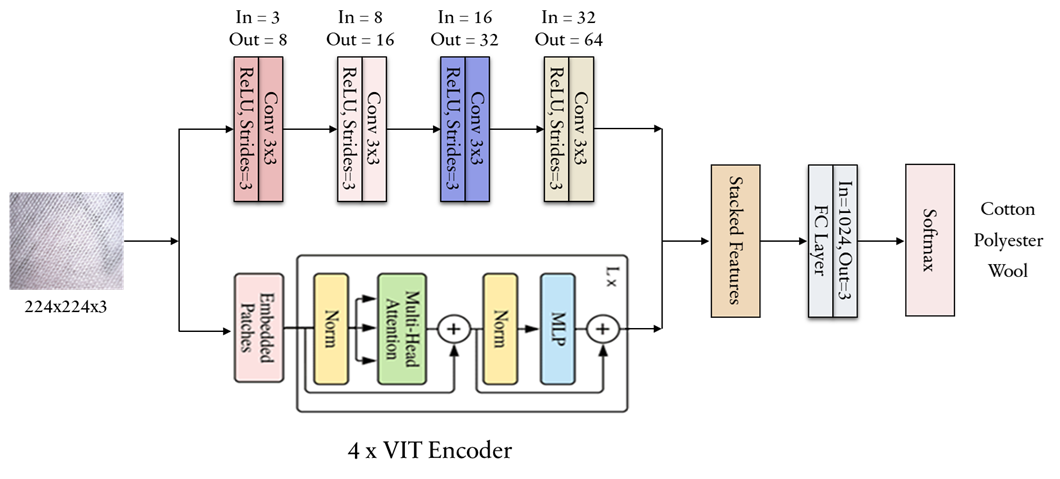
\includegraphics[width=0.8\textwidth]{images/ModelDiagram.png}
    \caption{Proposed hybrid deep learning architecture for fabric classification.}
    \label{fig:model_diagram}
\end{figure}

In parallel, the input image is divided into fixed-size patches and passed through a ViT branch. The Vision Transformer processes these patches using multi-head self-attention and feed-forward layers, which are effective in learning long-range dependencies and global spatial relationships. Each patch is embedded into a latent space with positional encodings and passed through a series of transformer encoders.

The feature maps generated by the CNN and ViT branches are then flattened and concatenated to form a unified feature vector. This fused representation is passed through a fully connected layer, followed by a softmax classifier to predict the fabric class.

The model is trained using the cross-entropy loss function with the Adam optimizer. Standard evaluation metrics such as accuracy, precision, recall, and F1-score are used to assess performance. This hybrid architecture allows the system to generalize well across fabric types with subtle visual differences, improving robustness in real-world applications.

\section*{Results}

The proposed hybrid CNN–ViT architecture was evaluated on fabric image datasets using standard classification metrics, including accuracy, precision, recall, and F1-score. The model was tested on both macro (RGB) fabric images and Optical Coherence Tomography (OCT) cross-sectional images. Experimental implementation was carried out using PyTorch, with training optimized using the Adam optimizer and a learning rate of 0.001.

On macro images, the model achieved a classification accuracy of 96.84\% for cotton, 99.63\% for polyester, and 98.09\% for wool. The precision and recall scores were consistently high across all classes, indicating balanced performance in identifying both common and visually similar fabrics.

On the OCT dataset, the model demonstrated exceptional results, achieving 99.66\% accuracy for cotton and perfect accuracy (100\%) for polyester and wool. Precision, recall, and F1-scores were all reported as 1.00, suggesting zero misclassifications in test samples.

Comparative analysis with existing models from the literature showed that the hybrid architecture outperformed individual CNN-based approaches like VGG-16~\cite{hong2020cnn} and even lightweight CNNs such as MobileNetV2~\cite{siam2021textilenet}. It also surpassed standalone ViT-based pipelines like those proposed by Chitra et al.~\cite{chitra2022vit}, validating the effectiveness of the dual-stream fusion strategy.

Overall, the results demonstrate that combining local feature extraction (CNN) with global attention modeling (ViT) yields a more robust and accurate solution for fabric classification, capable of handling variability in texture, structure, and imaging modality.

\section{Security Orchestration Automation and Response}

The increasing volume, velocity, and sophistication of cyber threats have made manual incident response insufficient in modern Security Operations Centers (SOCs). As organizations face growing pressure to detect and mitigate attacks in real time, Security Orchestration, Automation, and Response (SOAR) platforms have emerged as a critical solution for scaling security operations and reducing response times. SOAR systems integrate threat intelligence, automate repetitive tasks, and orchestrate incident handling workflows across various tools and teams~\cite{paloalto_soar, ibm_soc}.

This internship project, conducted at Bharat Electronics Limited (BEL), focuses on the design and implementation of a custom SOAR platform tailored for real-time cyber incident management. The platform includes core modules such as user authentication, an interactive dashboard, incident analytics, workflow automation, playbook execution, and integration with the MITRE ATT\&CK framework~\cite{mitre_attack}. The goal is to reduce Mean Time to Detect (MTTD) and Mean Time to Respond (MTTR) by enabling rapid triage and automated mitigation.

By integrating automation driven decision support with customizable workflows, this SOAR platform empowers security analysts to respond proactively to threats while minimizing fatigue and human error. The project aligns with industry best practices and addresses real-world challenges in enterprise-grade SOC environments.

\section*{Security Operations Center (SOC) and the Role of SOAR}

A Security Operations Center (SOC) is a centralized facility responsible for continuously monitoring, detecting, analyzing, and responding to cybersecurity incidents within an organization. SOC teams play a critical role in safeguarding information systems by managing security alerts, coordinating incident responses, and maintaining compliance with organizational and regulatory policies~\cite{ibm_soc}.

Typically, a SOC is staffed with multiple tiers of security analysts:
\begin{itemize}[noitemsep, topsep=0pt]
    \item \textbf{Tier 1 (Alert Analysts):} Responsible for monitoring alerts, triaging incidents, and escalating suspicious activities.
    \item \textbf{Tier 2 (Incident Responders):} Perform deeper investigations, validate threats, and initiate containment actions.
    \item \textbf{Tier 3 (Threat Hunters):} Conduct proactive threat hunting and in-depth forensic analysis.
\end{itemize}

\begin{figure}[htbp]
    \centering
    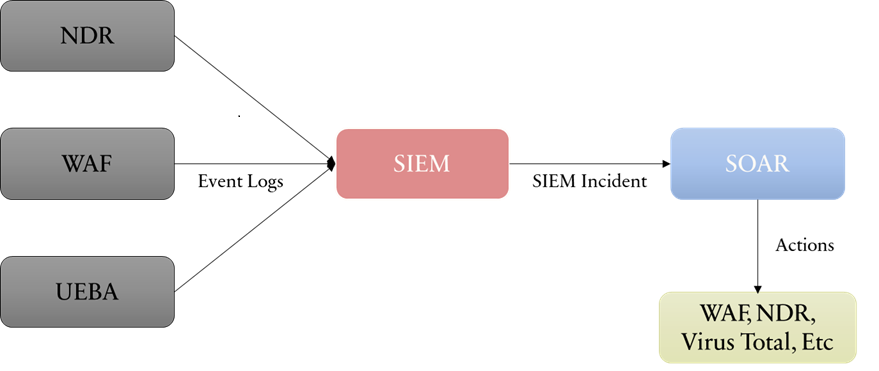
\includegraphics[width=0.85\textwidth]{images/data_flow_soc.png}
    \caption{Data flow in a typical Security Operations Center (SOC) environment.}
    \label{fig:data_flow_soc}
\end{figure}

However, as cyberattacks grow more sophisticated and the volume of alerts increases, traditional SOCs face challenges related to analyst fatigue, delayed response times, and inconsistent incident handling. This is where SOAR (Security Orchestration, Automation, and Response) platforms play a transformative role.

SOAR systems integrate with SIEM (Security Information and Event Management) tools, threat intelligence platforms, and endpoint security solutions to automate repetitive tasks, correlate events across systems, and trigger predefined playbooks. This reduces Mean Time to Detect (MTTD) and Mean Time to Respond (MTTR), while also ensuring standardization and auditability of incident response actions~\cite{paloalto_soar}.

In this project, the SOAR platform was designed to emulate real SOC workflows, enabling seamless analyst interaction, intelligent response orchestration, and alignment with the MITRE ATT\&CK framework~\cite{mitre_attack}, thereby enhancing the operational efficiency of the SOC environment.

\section*{SOAR Platform Components}
\addcontentsline{toc}{section}{SOAR Platform Components}

The custom SOAR platform developed during this internship consists of multiple integrated components designed to streamline and automate cybersecurity operations. Each module is built with a focus on usability, scalability, and alignment with real-world SOC workflows. The primary components are as follows:

\begin{enumerate}
    \item \textbf{User Authentication and Access Control:} 
    Implements secure login and registration with role-based access to differentiate between analysts, administrators, and managers.

    \item \textbf{Dashboard and Incident Analytics:} 
    Provides real-time visualizations including pie charts (severity, status), bar graphs (top events), and time-series graphs to track incident trends and mitigation rates.

    \item \textbf{Incident Management Module:} 
    Displays a dynamic table of security incidents enriched with deatils about the incident. Analysts can manually review, assign, and change incident statuses or let the system apply automated mitigation using machine learning.

    \item \textbf{Integrations Module:} 
    Enables external application integration via RESTful APIs. Users can configure apps (name, token, description) and their corresponding actions (endpoint, method, parameters).

    \item \textbf{Playbook Management:} 
    Supports creation and editing of automated response playbooks triggered by MITRE ATT\&CK technique IDs. Each playbook is mapped to workflows for seamless execution.

    \item \textbf{Workflow Builder:} 
    Offers a drag-and-drop interface to define logical sequences of actions using app nodes and edges. Analysts can design, execute, and track workflows in real time.

    \item \textbf{MITRE ATT\&CK Matrix Integration:} 
    Visualizes ATT\&CK techniques, allowing analysts to explore incident frequency and identify attack vectors. Techniques are color-coded based on activity density.

\end{enumerate}

These components collectively enable end-to-end incident response orchestration, minimize analyst fatigue, and improve SOC efficiency through intelligent automation.


\section*{Thesis Organization}

The thesis is organised in four chapters including the thesis introduction, detailed expationation of both the research work on fabric classification and internship on development of SOAR platform and the conclusion. Each chapter is structured to provide a comprehensive understanding of the respective topics, methodologies, and outcomes.

\textbf{Chapter 1: Introduction}  
This chapter provides an overview of the motivation, objectives, and scope of the thesis. It introduces the dual focus of the work, covering both the research and internship components.

\textbf{Chapter 2: Fabric Classification using Deep Learning}  
This chapter presents the research conducted on textile fabric classification using hybrid deep learning models. It includes the following sections:
\begin{itemize}[noitemsep, topsep=0pt]
    \item \textbf{Fibre and Fabric: Understanding the Distinction} – Explains the difference between fiber-level and fabric-level materials and their relevance to classification.
    \item \textbf{Literature Review} – Discusses related work in fabric classification that has utilized deep learning techniques. These works acts as a base for the proposed hybrid model.
    \item \textbf{Methodology} – Details the proposed hybrid CNN–ViT model architecture.
    \item \textbf{Experimental Setup and Results} – Describes the experimental configuration, and performance evaluation with the help of various metrics such as accuracy, precision, recall, and F1-score.
    \item \textbf{Conclusion and Future Work} – Summarizes key findings and proposes directions for continued research.
\end{itemize}

\textbf{Chapter 3: Security Orchestration, Automation, and Response (SOAR)}  
This chapter details the internship work undertaken at Bharat Electronics Limited (BEL) and includes the following sections:
\begin{itemize}[noitemsep, topsep=0pt]
    \item \textbf{Security Operations Center (SOC)} – Introduces the role and structure of SOCs in cybersecurity.
    \item \textbf{Data Flow in SOC} – Explains how data is ingested, processed, and acted upon within a SOC.
    \item \textbf{Security Information and Event Management (SIEM) in SOC} – Describes the function of SIEM tools in correlating and generating security alerts.
    \item \textbf{SIEM Incident Flow to SOAR} – Illustrates the integration and transition of incidents from SIEM to the SOAR platform.
    \item \textbf{SOAR Platform Components} – Details the modules developed for the SOAR platform including incident management, playbooks, workflows, and MITRE ATT\&CK integration.
    \item \textbf{Future Work} – Discusses potential enhancements and scalability considerations for the SOAR platform.
\end{itemize}

\textbf{Chapter 4: Conclusion}  
The final chapter summarizes the contributions made in both parts of the thesis and reflects on their broader implications. It also highlights future research and development opportunities.


% \part{Security Orchestration Automation and Response}

% References
\baselineskip=16pt	% Length between two lines in a paragraph

\addcontentsline{toc}{section}{References}
\bibliographystyle{unsrt}
\renewcommand{\bibname}{References}
\bibliography{synopsis_contents/references}

\end{document}